\begin{lstlisting}[frame=lines,style=Matlab-editor]
clear;close all;clc

% Constants
c.m = 0.25; % kg
c.k = 25; % N/m
c.l = 0.5; % m
c.I = (1/3)*c.m*c.l^2; %kg.m^2
c.g = 9.81; % m/s^2

syms l g m k I theta phi thetadot thetaddot phidot phiddot...
    An At Cn Ct

% Cartesian locations of bar ends
b = l*[sin(theta);-cos(theta)];
d = l*[sin(phi)+1;-cos(phi)];
rbd = d - b;
rbdSquared = rbd.^2;
% Spring Length (mag)
ls = simplify(rbdSquared(1) + rbdSquared(2))^(1/2);
% Spring Direction (Left and Right)
ehatsL = (d - b) / ls;
ehatsR = (b - d) / ls;
% Normal / Tangential for Theta
ehatnT = [-sin(theta);cos(theta)];
ehattT = [cos(theta);sin(theta)];
% Normal / Tangential for Phi
ehatnP = [-sin(phi);cos(phi)];
ehattP = [cos(phi);sin(phi)];
% Spring Force (Left and Right)
FsL = k*(ls-l)*ehatsL;
FsR = k*(ls-l)*ehatsR;

% Spring force in normal direction (Theta)
Fs_nT = simplify(FsL(1)*ehatnT(1)+FsL(2)*ehatnT(2));
% Spring force in tangential direction (Theta)
Fs_tT = simplify(FsL(1)*ehattT(1)+FsL(2)*ehattT(2));

% Spring force in normal direction (Phi)
Fs_nP = simplify(FsR(1)*ehatnP(1)+FsR(2)*ehatnP(2));
% Spring force in tangential direction (Phi)
Fs_tP = simplify(FsR(1)*ehattP(1)+FsR(2)*ehattP(2));

% Sum of Normal Forces, left bar (Theta)
eqn(1) = m*(l/2)*thetadot^2 == Fs_nT + An - m*g*cos(theta);
% Sum of Tangential Forces, left bar (Theta)
eqn(2) = m*(l/2)*thetaddot == Fs_tT + At - m*g*sin(theta);
% Sum of Moments, left bar (Theta)
eqn(3) = -(l/2)*(m*g*sin(theta)) + (Fs_tT)*(l) == (1/3)*m*(l^2)*thetaddot;

% Sum of Normal Forces, right bar (Phi)
eqn(4) = m*(l/2)*phidot^2 == Fs_nP + Cn - m*g*cos(phi);
% Sum of Tangential Forces, right bar (Phi)
eqn(5) = m*(l/2)*phiddot == Fs_tP + Ct - m*g*sin(phi);
% Sum of Moments, right bar (Phi)
eqn(6) = -(l/2)*(m*g*sin(phi)) + (Fs_tP)*(l) == (1/3)*m*(l^2)*phiddot;

x = solve(eqn,[thetaddot,phiddot,An,At,Cn,Ct]);

syms theta(t) thetadot(t) phi(t) phidot(t)

thetaEOM = subs(x.thetaddot, {'theta', 'thetadot'}, {theta, thetadot});
phiEOM = subs(x.phiddot, {'phi', 'phidot'}, {phi, phidot});

eom = odeFunction([thetadot; thetaEOM; phidot; phiEOM],...
    [theta; thetadot; phi; phidot],m,k,l,I,g);

theta_o = [pi/12 -pi/12 pi/36];

for i = 1:3
    [T,S] = ode45(@(t,s)eom(t,s,c.m,c.k,c.l,c.I,c.g),linspace(0,10,1001),...
        [theta_o(i),0,pi/12,0]);
    figure
    hold on
    grid on
    xlabel('Time, sec')
    ylabel('Angular Position, rad')
    plot(T,S(:,1),'DisplayName', ['\theta_o = ' num2str(rad2deg(theta_o(i))) '^o'])
    plot(T,S(:,3),'DisplayName', '\phi_o = 15^o')
    legend('show')
end

% Checking EOM Units
u = symunit;
m = m*u.kg;
g = g*u.m/u.s^2;
l = l*u.m;
k = k*u.N/u.m;
An = An*u.N;
At = At*u.N;
Cn = Cn*u.N;
Ct = Ct*u.N;
theta = 'theta';
thetadot = 'thetadot'/u.s;
thetaddot = 'thetaddot'/u.s^2;
phi = 'phi';
phidot = 'phidot'/u.s;
phiddot = 'phiddot'/u.s^2;

eqn = subs(eqn);
unitCheck = checkUnits(eqn)
\end{lstlisting}
\color{gray} \begin{verbatim}
unitCheck =
  struct with fields:

    Consistent: [1 1 1 1 1 1]
    Compatible: [1 1 1 1 1 1]
\end{verbatim} \color{black}
\center
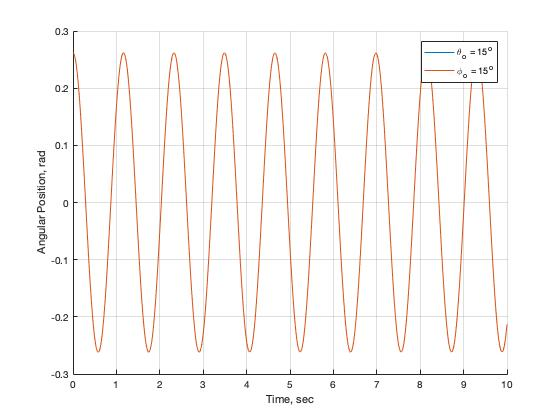
\includegraphics[center,width=4in]{rigid_01}

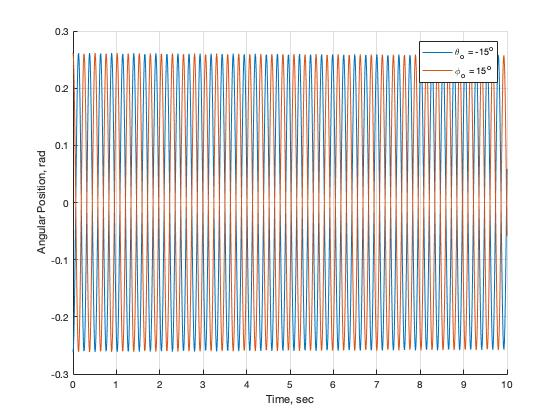
\includegraphics[center,width=4in]{rigid_02}

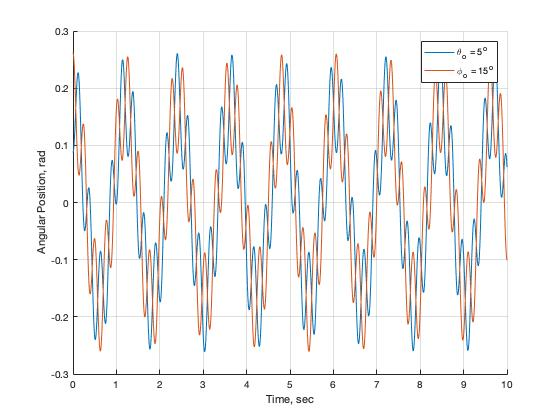
\includegraphics[center,width=4in]{rigid_03}
